% !TeX spellcheck = en_US
\documentclass[french]{yLectureNote}

\title{Optique ondulatoire}
\subtitle{Physique}
\author{Paulhenry Saux}
\date{\today}
\yLanguage{Français}

\professor{F.Pettinari}
\usepackage{graphicx}%----pour mettre des images
\usepackage[utf8]{inputenc}%---encodage
\usepackage{geometry}%---pour modifier les tailles et mettre a4paper
%\usepackage{awesomebox}%---pour les boites d'exercices, de pbq et de croquis ---d\'esactiv\'e pour les TP de PC
\usepackage{tikz}%---pour deiffner + d\'ependance de chemfig
% \usepackage{tabularx}%---pour dimensionner automatiquement les tableaux avec variable X
\usepackage{awesomebox}%---Pour les boites info, danger et autres
\usepackage{menukeys}%---Pour deiffner les touches de Calculatrice
\usepackage{fancyhdr}%---pour les en-t\^ete personnalis\'ees
\usepackage{blindtext}%---pour les liens
\usepackage{hyperref}%---pour les liens (\`a mettre en dernier)
\usepackage{caption}%---pour la francisation de la l\'egende table vers Tableau
\usepackage{pifont}
\usepackage{array}%---pour les tableaux
\usepackage{lipsum}
\usepackage{yFlatTable}
\usepackage{multicol}
\newcommand{\Lim}[1]{\lim\limits_{\substack{#1}}\:}
\renewcommand{\vec}{\overrightarrow}
\newcommand{\N}[0]{\mathbb{N}}
\newcommand{\dd}{\mathrm{d}}
\newcommand{\norm}[1]{||\vec{#1}||}
\newcommand{\fo}{\psi(\vec{r},t)}
\newcommand{\foe}{\psi(\vec{r},t)\*}
\newcommand{\HH}{\hat{H}}
\newcommand{\hb}{\hbar}
\newcommand{\lap}{\nabla^2}
\newcommand{\lapcc}{\frac{\partial^2 }{\partial x^2}+\frac{\partial^2 }{\partial y^2}+\frac{\partial^2 }{\partial z^2}}
\newcommand{\mpsi}{\(\psi\)}
\newcommand{\und}{\underline}
\newcommand{\dph}{\Delta\varphi}
\begin{document}
\chapter{TP d'optique}
\section{Diffraction et interférences 1}
\subsection{Diffraction}
\subsubsection{Description du montage expérimental}
On place après le faisceau laser (1) la fente diffractante (2), la lentille de focale 0.5m (3), puis la photodiode (4) placée sur un pied à déplacement transversal, sur le foyer image de la lentille. La photodiode est connectée au Voltmètre. L'ensemble est aligné verticalement.
\begin{center}
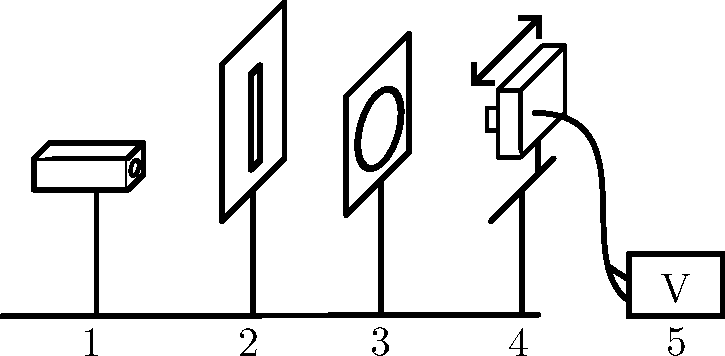
\includegraphics[scale=0.4]{1_1}
\end{center}
\subsection{À savoir}
\begin{itemize}
 \item lorsque la photodiode n'est pas éclairée par le laser, la valeur de tension renvoyée n'est pas nulle. Elle est d'environ 20 mV. Il faut donc rajouter une constante C à la formule donnée pour la modélisation.
\end{itemize}
\subsection{Interférences}
\subsubsection{Description du montage expérimental}
On place après le faisceau laser (1) un objectif de microscope (2), puis le prisme (3) à une distance l de cet objectif. L'objectif sera positionné à une distance de 2m de l'écran d'Observation. On mesure sur l'écran à l'aide du papier millimétré la distance entre une dizaine de frange d'intéférence et on releve le nombre exact de frange compris dans la mesure.
\begin{center}
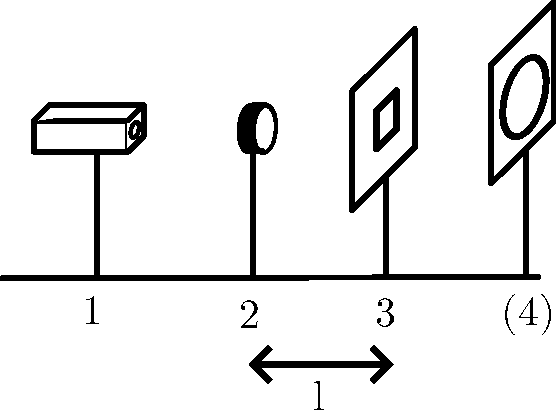
\includegraphics[scale=0.4]{1_2}
\end{center}
\subsection{À savoir}
\begin{itemize}
 \item $i = \frac{d}{N}$
 \item $i = \frac{\lambda D}{a}$ avec D la Distance entre la source et l'écran et a la distance entre les 2 sources à l'origine des interférence
 \item $\theta = \frac{a}{2l}$ avec  \(l\), la distance entre la source et le prisme, \(a\), la distance entre les 2 sources virtuelles et \(\theta\), l'angle du prisme
 \item En posant une lentille L après le prisme : $ \gamma = \frac{EL}{LP} = \frac{a'}{a}$ avec avec \(a'\) la taille de l'image réelle des 2 sources virtuelles.
\end{itemize}
\section{Diffraction et interférences 2}
La lampe à mecure (1) est déjà positionnée. Nous alignons d'abord le trou source (2) avec l'occulaire (6). Puis avec la méthode d'autocollimation, nous plaçons la première lentille (4) de façon à ce que le trou source se trouve au foyer objet de cette dernière. Nous n'oublions le filtre (3) (le cas échéant) Nous plaçons ensuite la deuxième lentielle (5) de façon à ce que son foyer image se trouve dans l'occulaire. Enfin, nous plaçons l'objet diffractant (7) entre les 2 lentilles, son emplacement exact étant sans importance.
\begin{center}
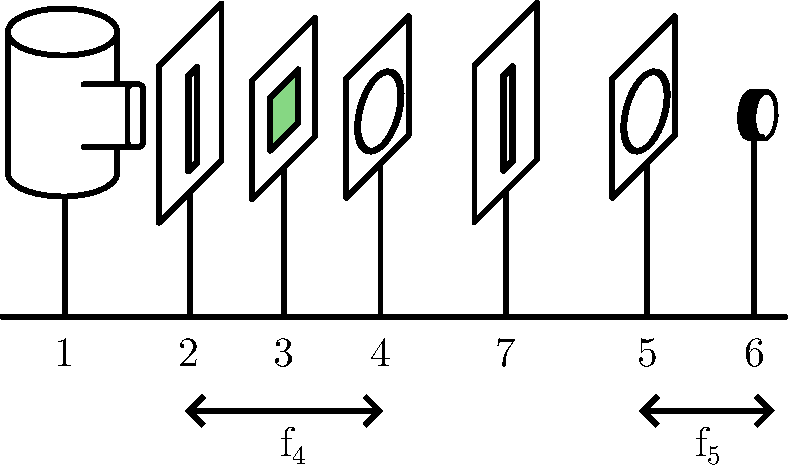
\includegraphics[scale=0.4]{2_1}
\end{center}
\subsection{À savoir}
\begin{itemize}
 \item $i = \frac{\lambda f}{a}$ avec f la focale de la deuxième lentille.
 \item \(L = \frac{2\lambda f}{a}\), avec a la largeur de la fente et L la largeur de la tache centrale
\end{itemize}
\section{Réseau}
\subsection{Montage expérimental}
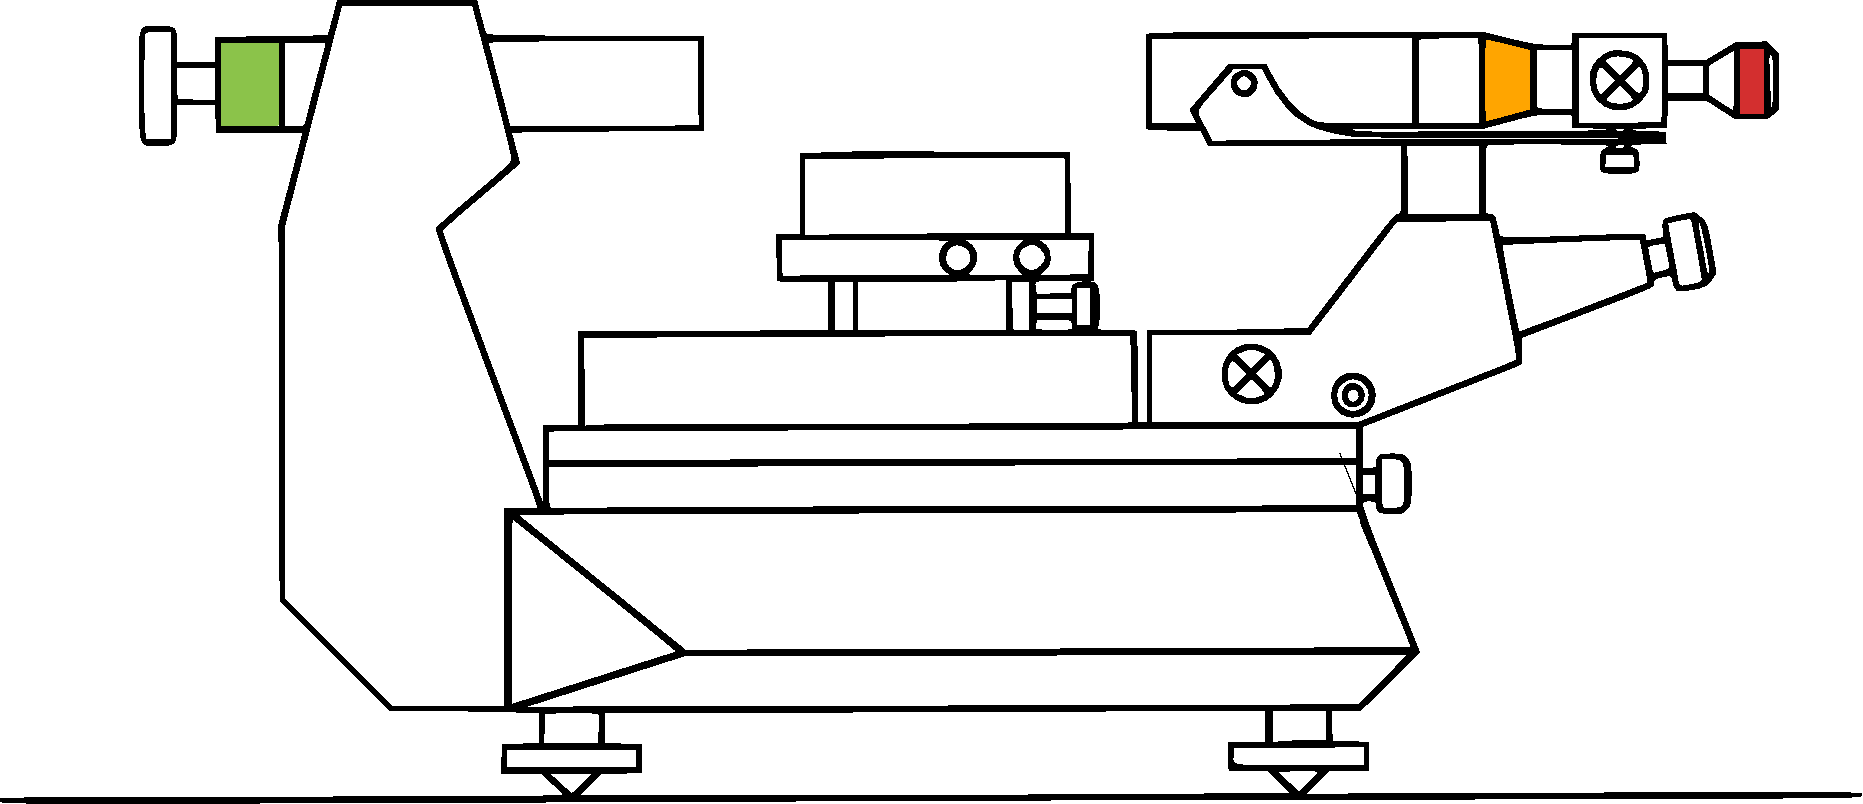
\includegraphics[scale=0.3]{gonio}

On règle d'abord la lunette :
\begin{enumerate}
 \item {\color{criticalColor}Réglage de l'oculaire} : on règle la distance oculaire/réticule (en tirant plus où moins l’oculaire) de façon à voir net le
réticule sans accommoder, ce dernier se trouve alors dans le plan focal objet de l'oculaire, donc son image à l’infini pour l’œil.
\item {\color{warningColor}Réglage de l'objectif} : il s’agit ici de régler la distance objectif/réticule de façon à ce que l'image d'un objet à l'infini se
forme dans le plan focal image de l'objectif, soit dans le plan du réticule. il s’agit que le réticule et son image ne se déplacent pas l'un par rapport à l'autre lorsque
l'œil se déplace transversalement (hochements de tête) de façon à éviter l'erreur de parallax
\end{enumerate}
On règle ensuite le {\color{informationColor}collimateur} : Il permet d'obtenir un objet (fente) à l'infini.
Il comporte une lentille et la distance
fente/lentille doit être réglée pour
que le collimateur donne un faisceau de
rayons parallèles, c'est-à-dire pour que la
fente soit dans le plan focal objet de la
lentille.

On règle ensuite le 0 du goniomètre : il s'agit de faire concider le réticule et la raie centrale émise.
\subsection{À savoir}
\begin{itemize}
 \item Relation des réseaux : \(\sin(\theta_d)-\sin(\theta_i) = kN\lambda = k\lambda\frac{1}{p}\)
 \item On mesure \(\theta_d\) à partir de la position de \(\theta_i\)
 \item L'ordre est compté à partir de la normale de l'incidence.
 \item Minium de déviation : \(D_m = \frac{Y_1-Y_2}{2}\)
 \item Formule de la déviation : \(2\sin(\frac{D_m}{2}) = kN\lambda\)
 \item Il faut faire attention à la convention de signe théorique qui est différente de celle du goniomètre
 \item Les valeurs de N théoriques sont \( 590 551\)/m pour le réseau  à 15 000 et le double pour le réseau à 30 000 fentes par inch.
 \item Dans Regressi, bien régler le type d'angle utilisé (degré ou radian)
\end{itemize}


 \end{document}
